\documentclass[border=9pt]{standalone}
\usepackage[fontset=fandol]{ctex}
\usepackage{amsmath,amssymb,tikz}
\usetikzlibrary{arrows.meta,calc,decorations.pathmorphing}
\tikzset{arr/.style={-{Stealth[length=2mm]},semithick}}
\begin{document}

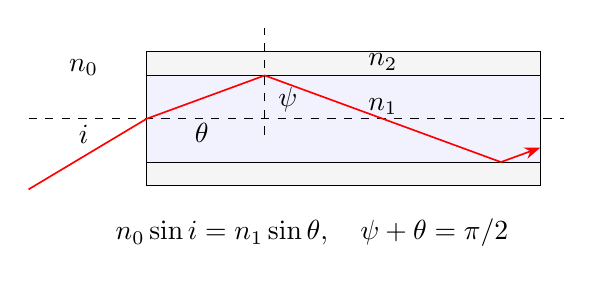
\begin{tikzpicture}[scale=1]
\draw[fill=gray!8] (0,-.85) rectangle(5,.85);
\draw[fill=blue!5] (0,-.55) rectangle(5,.55);
\draw[dashed] (-1.5,0)--(5.3,0);
\draw[arr,red] (-1.5,-.897)--(0,0)--(1.5,.55)--(4.5,-.55)--(5,-.3667);
\draw[dashed] (1.5,-.2)--(1.5,1.15);
\node at (-.8,-.2) {$i$};
\node at (.7,-.18) {$\theta$};
\node[right] at (1.55,.25) {$\psi$};
\node at (3,.15) {$n_1$}; \node at (3,.72) {$n_2$};
\node at (-.8,.65) {$n_0$};
\node at (2.1,-1.45) {$n_0\sin i=n_1\sin\theta,\quad\psi+\theta=\pi/2$};
\end{tikzpicture}

\end{document}
